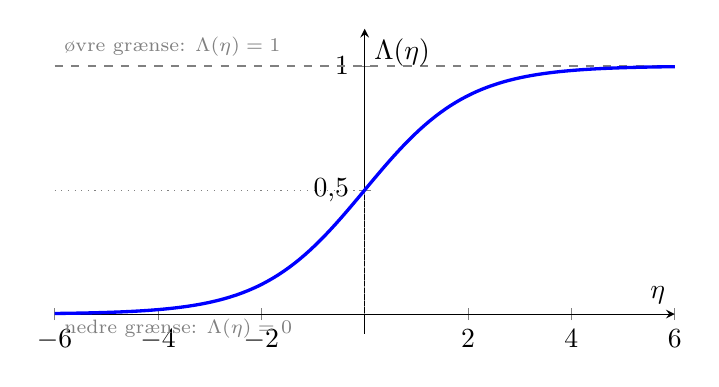
\begin{tikzpicture}
\begin{axis}[
    width=0.78\textwidth,
    height=0.45\textwidth,
    xlabel={$\eta$},
    ylabel={$\Lambda(\eta)$},
    xmin=-6, xmax=6,
    ymin=-0.08, ymax=1.15,
    axis lines=middle,
    ytick={0.5,1},
    yticklabels={{0{,}5},{1}},
    xtick={-6,-4,-2,2,4,6},
    domain=-6:6,
    samples=120,
    clip=false
]
\addplot[dashed, gray, thick] coordinates {(-6,1) (6,1)};
\addplot[dotted, gray] coordinates {(-6,0.5) (0,0.5)};
\addplot[dotted, gray] coordinates {(0,0) (0,0.5)};
\addplot[very thick, blue] {1/(1+exp(-x))};
\node[anchor=south west, font=\scriptsize, gray] at (axis cs:-6,1) {øvre grænse: \(\Lambda(\eta)=1\)};
\node[anchor=north west, font=\scriptsize, gray] at (axis cs:-6,0.02) {nedre grænse: \(\Lambda(\eta)=0\)};
\end{axis}
\end{tikzpicture}
